%Standardní zobrazovací řetězec a realizace jeho jednotlivých kroků. Gouraudovo a Phongovo stínování. Řešení viditelnosti. Grafický standard OpenGL: stručná charakteristika.
\subsection{Standardní zobrazovací řetěz}
\begin{itemize}
	\item Klade důraz na rychlost nikoli na kvalitu.
	\item Realizuje ho OpenGL, (dire).
\end{itemize}
\begin{figure}[H]
\centering
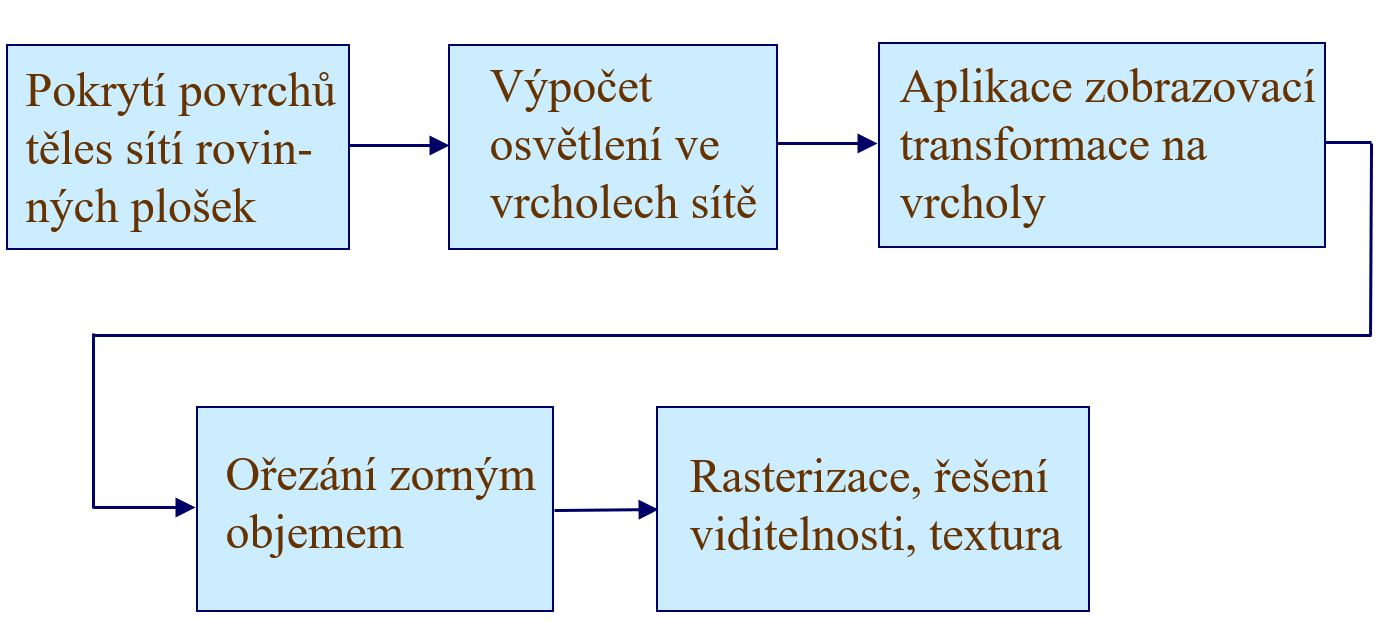
\includegraphics[width=0.8\textwidth]{assets/5_retezec}
\end{figure}

\begin{itemize}
	\item  \textbf{Pokrytí povrchu objektů sítí rovinných plošek:}
	\begin{itemize}
		\item Ploškami bývají nejčastěji trojúhelníky nebo čtyřúhelníky.
		\item Pro objekty ve tvaru mnohostěnu je takové dělní vcelku samozřejmé.
		\item K přesnějšímu výpočtu barev bývá, ale někdy dělení na plošky jemnější.
		\item Někdy síť rovinných plošek žádaný povrch pouze aproximuje.
	\end{itemize}
	\item \textbf{Výpočet osvětlení ve vrcholech sítě}
	\item k tomu známe:
	\begin{itemize}
		\item Polohu, intenzitu a barvu světelných zdrojů.
		\item Souřadnice vrcholů ($P$), normál ($n$) a konstanty popisující optické vlastnosti materiálu ($O_a, O_d, O_s$)
		\begin{figure}[H]
		\centering
		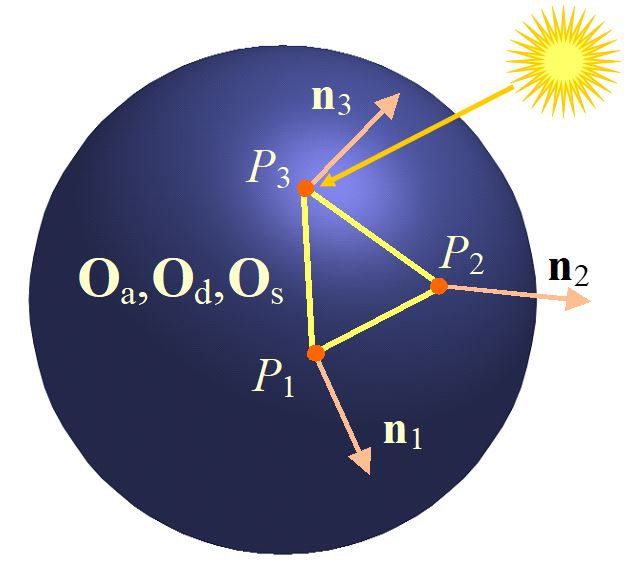
\includegraphics[width=0.5\textwidth]{assets/5_vypocet_barevneho_vjemu}
		\end{figure}
	\end{itemize}
	\item \textbf{Aplikace zobrazovací transformace na vrcholy}
	\begin{itemize}
		\item Oblíbenou technikou je středové promítání. To je zadáno:
		\begin{itemize}
			\item Polohou průmětny.
			\item Polohou středu promítání.
		\end{itemize}
		\begin{figure}[H]
		\centering
		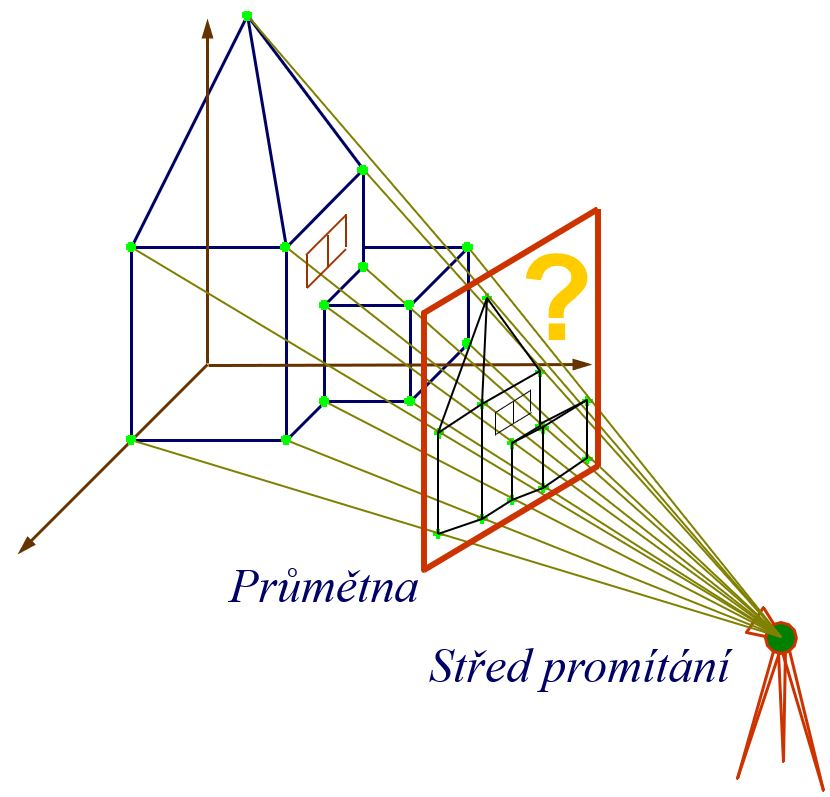
\includegraphics[width=0.5\textwidth]{assets/5_stred_promitani}
		\end{figure}
	\end{itemize}
	\item \textbf{Ořezání zorným objemem}
	\begin{itemize}
		\item Objekty nebo jejich části, nacházející se mimo zorný objem (obvykle jehlan) jsou odstraněny.
	\end{itemize}
		\begin{figure}[H]
		\centering
		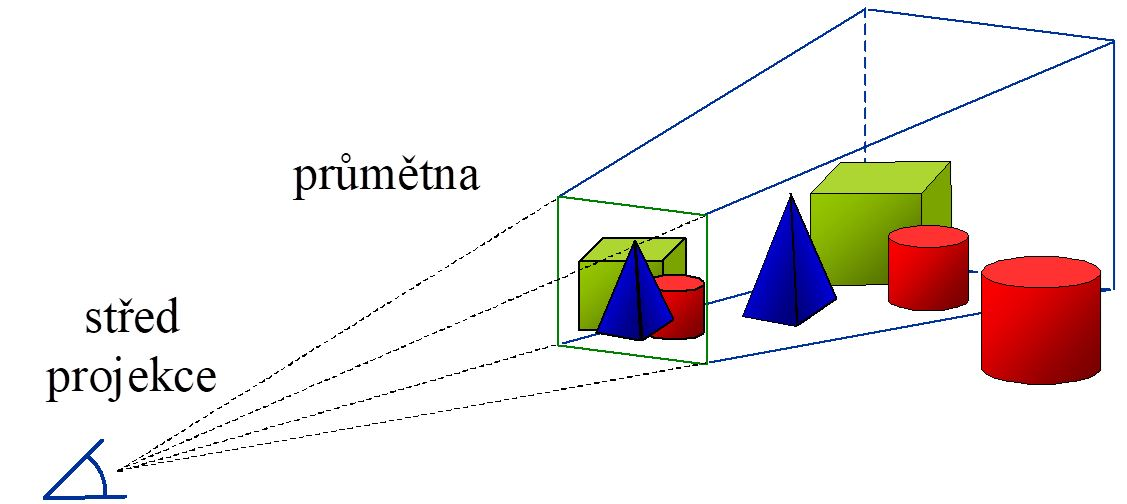
\includegraphics[width=0.5\textwidth]{assets/5_orezani_zornym_pole}
		\end{figure}
	%\begin{itemize}
	\item \textbf{Rasterizace plošek}
	\begin{itemize}
		\item Postupně zpracovávány všechny plošky.
		\item Pro každou plošku rozsvěceny všechny její pixely.
		\item Barva každého pixelu se stanoví interpolací mezi hodnotami ve vrcholech.
		\begin{figure}[H]
		\centering
		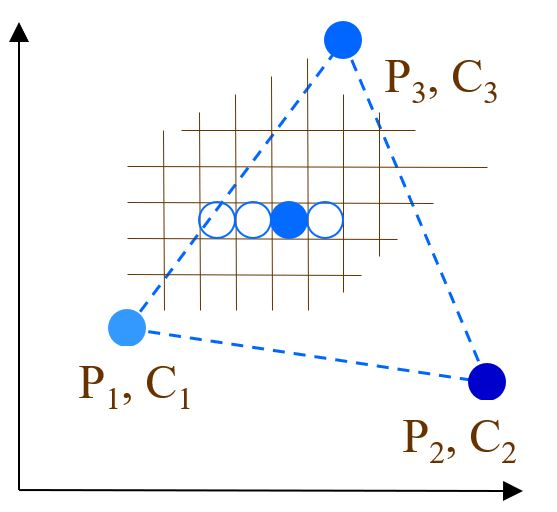
\includegraphics[width=0.5\textwidth]{assets/5_rasterizace_plosek}
		\end{figure}
	\end{itemize}
	\item \textbf{Řešení viditelnosti (z--buffer)}
	\begin{itemize}
		\item Pro rozhodnutí viditelnosti se použijí hodnoty souřadnice $z$ (zde je $z_1 > z_2$).
		\item Před řešením viditelnosti bývá centrálním promítání převedeno na rovnoběžné.
		\begin{figure}[H]
		\centering
		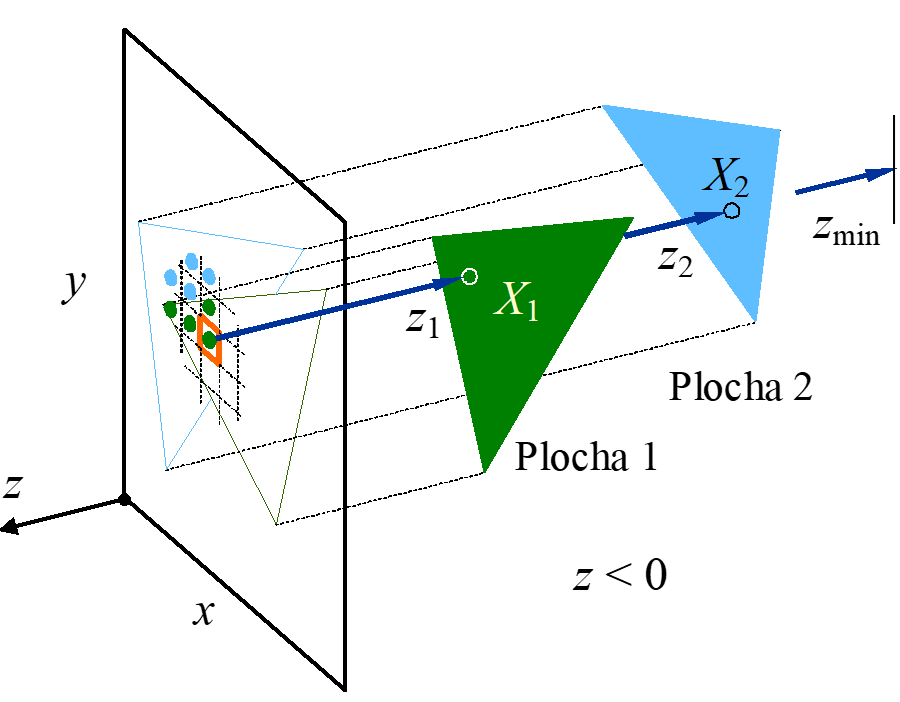
\includegraphics[width=0.5\textwidth]{assets/5_pip_zbuffer}
		\end{figure}
	\end{itemize}
	\item \textbf{Nanášení textury}
	\begin{itemize}
		\item Vzhled obrázků lze vylepšit nánášením textury.
	\end{itemize}
\end{itemize}
\subsection{Stínování (shading)}
\begin{itemize}
	\item Vykreslování barevných objektů různými odstíny barev.
	\item Lze odlišit křivosti ploch a tím docílit lepšího prostorového vjemu.
	\item Neplést s výpočtem vrženého stínu.
	\item Základní typy: Konstantní stínování, Gouraudovo stínování (Interpolace barvou), Phongovo stínování (Interpolace normálových vektorů)
\end{itemize}
\subsection{Gouraudovo stínování (Interpolace barvou)}
Princip metody spočívá v tom, že pokud budeme znát normálu v každém vrcholu každé plochy objektu, pak lze vypočítat barvu v tomto vrcholu a interpolací vypočítat barvu pixelu uvnitř plošky (bilineární interpolace).

Přesto ani tento způsob stínování neposkytuje zcela věrný obraz reálných objektů - interpolace samotného odstínu barvy totiž nemůže způsobit místní zvýšení jasu na plošce, stejně jako nemůže kvalitně vytvořit odlesky způsobené odraženým světlem. Dá se říci, že tato metoda zahlazuje barevné rozdíly u místních nerovností povrchu.

Normálový vektor $n_r$ vypočteme jako aritmetický průměr vektorů okolních plošek.
		\begin{figure}[H]
		\centering
		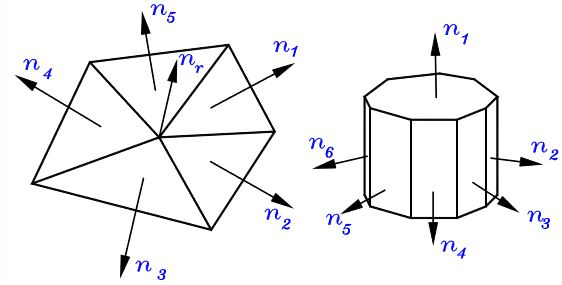
\includegraphics[width=0.5\textwidth]{assets/5_gouraud}
		\end{figure}

\begin{itemize}
	\item Vypočteme normálové vektory pro všechny plošky ze kterých je objekt složený.
	\item Pro každý vrchol spočítáme normálový vektor v tomto vrcholu jako průměr normálových vektorů plošek, které se v tomto vrcholu stýkají.
	\item Z normálových vektorů ve vrcholech a pozice světelného zdroje vypočteme barvy ve vrcholech plošek.
	\item Provedeme interpolaci barvy pro body jednotlivých plošek.
\end{itemize}
		\begin{figure}[H]
		\centering
		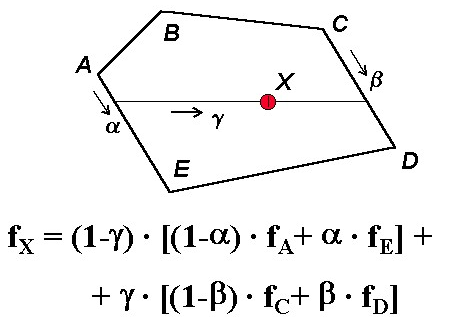
\includegraphics[width=0.5\textwidth]{assets/5_gouradovo}
		\end{figure} 
		\subsubsection*{Výhody}
			\begin{itemize}
				\item[$+$] umožnuje dobře zobrazit i hladké objekty,
				\item[$+$] používá se jako nejčastější metoda stínování.
			\end{itemize}
		\subsubsection*{Nevýhody}
			\begin{itemize}
				\item[$-$] nevnikají ostré odlesky uprostřed polygonů.
			\end{itemize}
\subsection{Phongovo stínování (Interpolace normálových vektorů)}
\begin{itemize}
	\item Interpolaci provádíme po řádcích.
	\item Touto metodou se odstraní problém neostrých odlesků.
	\item Je ale bohužel náročná na výpočet.
	\item Pro normálové vektory lze psát:
		\begin{equation*} 
		\begin{array}{c}
			n_A = n_1 + (n_2 - n_1) \cdot u; u <0, 1>, \\
			n_B = n_1 + (n_3 - n_1) \cdot w; w <0, 1>, \\
			n_Q = n_A + (n_B - n_A) \cdot t; t <0, 1>, \\
		\end{array}
		\end{equation*}
\end{itemize}
		\begin{figure}[H]
		\centering
		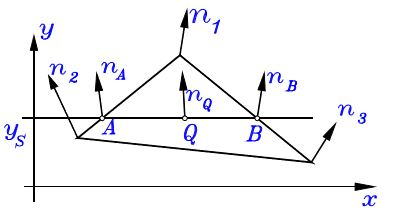
\includegraphics[width=0.5\textwidth]{assets/5_phong_stin}
		\end{figure}
\subsection{Řešení viditelnosti}
\begin{itemize}
	\item Podle výsledných dat
	\begin{itemize}
		\item \textbf{Vektorové algoritmy} -- geometrické prvky vrcholy, hrany a stěny. Výstupem je vektorové řešení.
		\item \textbf{Rastrové algoritmy} -- výsledkem je rastrový obraz (jednotlivé pixely obsahují barvu), většina současných metod.
	\end{itemize}
	\item Podle místa řešení
	\begin{itemize}
		\item \textbf{Řešení v prostoru objektů} -- proovnávání vzájemné polohy těles $0(n^2)$
		\item \textbf{Řešení v prostoru obrazu} -- pracujeme s promítnutými a rasterizovanými objekty. Pro pixely hledáme nejbližší objekty.
	\end{itemize}
\end{itemize}
Rastrové algoritmy:
\begin{itemize}
	\item \textbf{Malířův algoritmus} (Painter's algorithm) -- porovnává plochy z hlediska jejich $z$--tových souřadnic (plocha s menší $z$--tovou souřadnící bude kreslena první), jestliže se plochy \textbf{nepřekrývají}, potom na pořadí kresby nezáleží, pokud se protínají -- rozdělit na nepřekrývající se plochy.
		\begin{figure}[H]
		\centering
		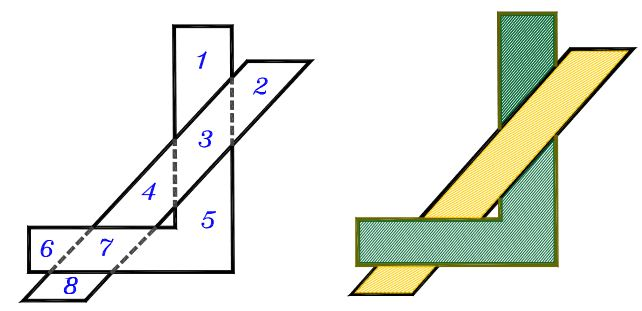
\includegraphics[width=0.5\textwidth]{assets/5_malir}
		\end{figure}
	\item \textbf{Dělení obrazovky }(Warnock subdivision)
		\begin{enumerate}
				\item Všechny plošky leží mimo zónu - zůstane barva pozadí. (a) 
				\item Oblast obsahuje právě jeden celý n-úhelník. Daná oblast se vyplní barvou a zbytek -pozadím. (b) 
				\item Oblast protíná právě jeden n-úhelník. Daná část se vyplní barvou, zbytek pozadí. (c) 
				\item Pokud zobrazovaná část je celá uvnitř jednoho n-úhelníka, potom se celá oblast zobrazí barvou nejbližšího n-úhelníka, který oblast obklopuje. (d) 
				\item Pokud nenastane jeden z vyjmenovaných případů - oblast se rozdělí.
		\end{enumerate}
		\begin{figure}[H]
		\centering
		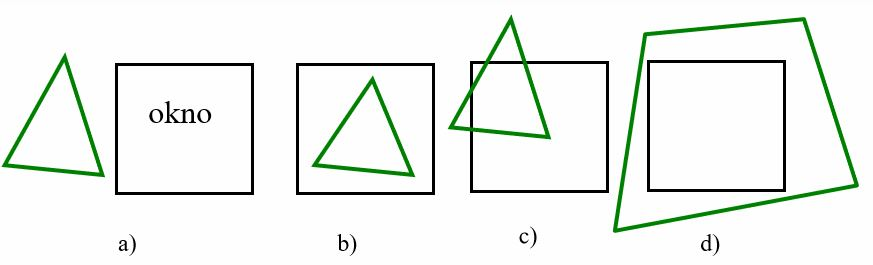
\includegraphics[width=0.5\textwidth]{assets/5_warnock}
		\end{figure}
	\item \textbf{Plovoucí horizont} (Floating Horizon Algorithm) -- metoda \uv{zig--zag}, počítáme od \uv{nejbližšího} rohu plochy k \uv{oku} pozorovatele.
		\begin{figure}[H]
		\centering
		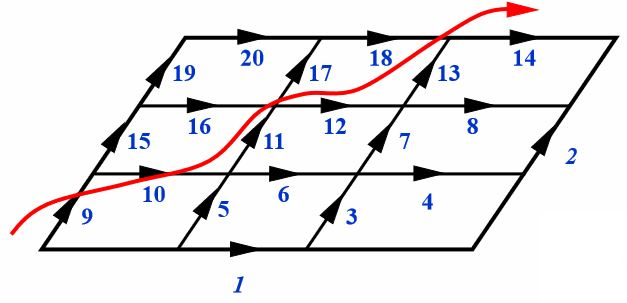
\includegraphics[width=0.5\textwidth]{assets/5_horizont}
		\end{figure}
	\item \textbf{Paměť hloubky} (\textbf{Z--buffer}, depth--buffer)
	\begin{enumerate}
				\item Vyplň obrazovou paměť barvou pozadí.
				\item Vyplň paměť hloubky -- nekonečnem
				\item Pro každou plochu najdi její průměť (rasterizaci) nalezenému pixelu $[x_i,y_i]$ přiřaď hloubku $z_i$
				\item Porovnej hloubku a zapiš do paměti 
	\end{enumerate}
		\begin{figure}[H]
		\centering
		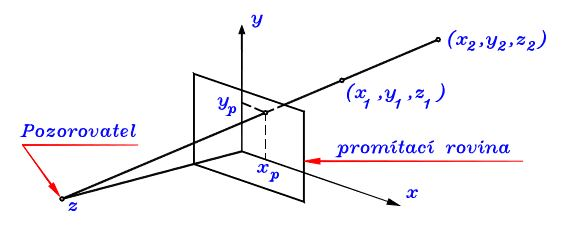
\includegraphics[width=0.7\textwidth]{assets/5_zbuffer}
		\end{figure}
		\begin{itemize}
		\item Nejznámější a nejefektivnější metoda.
		\item Každá plocha se zpracovává pouze jednou.
		\item Doba zpracování roste s počtem ploch lineárně (záleží i na velikosti ploch).
		\item Není potřeba žádné třídění nebo pomocné datové struktury.
		\item Možnost paralelních procesů.
		\end{itemize}
	\item Z--buffer -- paměť hlouby -- průhlednost - princip
	\begin{enumerate}
		\item Inicializuj color buffer a depth buffer.
		\item Postupně načti všechny plochy, neprůhledné zpracuj, průhledné si zapamatuj a odlož pro následné zpracování.
		\item Po zpracování neprůhledných ploch setřiď průhledné plochy podle vzdálenosti.
		\item Zpracuj průhledné plochy s použitím alfa míchání.
	\end{enumerate}
\end{itemize}
\subsection{Grafický standard OpenGL: stručná charakteristika}
OpenGL (Open Graphics Library) je grafická multiplatformní knihovna pro \textbf{tvorbu} a \textbf{zobrazování 2D a 3D objektů} vyvinutá firmou SGI (Silicon Graphics Inc.) v 90.letech. Dnes jde o všeobecně uznávaný \textbf{standard} podporován výrobci grafických karet. Standard OpenGL definuje množinu funkcí, které se volají z programu. Pokud nejsou některé z těchto funkcí podporovány na technické úrovni, je podpora realizována programově, což zajišťujě široké využití i při zachování techniceké nezávislosti programu. 

Používá se pro tvorbu \textbf{PC her}, \textbf{CAD programů}, aplikací \textbf{virtuální reality} či \textbf{vědeckotechnické vizualizace} apod. 

OpenGL je jednoduchý, \textbf{nepodporuje objektově orientované programování}. Přesto nabízí široké možnosti a urychluje práci s grafikou. Kromě vykreslování základních typů objektů, umožňuje OpenGL transformace. A to \textbf{transformace zobrazovací} a \textbf{transformace modelovací}. Při těchto transformací se pracuje s transformačními maticemi.

Na některých platformách je možné rozdělení aplikace na dvě relativně samostatné části – \textbf{serverovou} a \textbf{klientskou}. Při vykreslování se potom jednotlivé příkazy (což jsou většinou parametry funkcí OpenGL) přenášejí přes síťové rozhraní. Knihovna OpenGL (narozdíl od IRIS GL nebo Direct 3D) byla vytvořena tak, aby byla \textbf{nezávislá} na použitém operačním systému, grafických ovladačích a správcích oken (Window Managers). Proto také neobsahuje žádné funkce pro práci s okny (otevírání, zrušení, změnu velikosti), pro vytváření grafického uživatelského rozhraní (Graphical User Interface – GUI) ani pro zpracování událostí

Pro dosažení co největší nezávislosti na použité platformě zavádí knihovna OpenGL vlastní primitivní datové typy, například \textbf{GLbyte}, \textbf{GLint} nebo \textbf{GLdouble}.

Programátorské rozhraní knihovny OpenGL je vytvořeno tak, aby knihovna byla použitelná v téměř libovolném programovacím jazyce. Primárně je k dispozici hlavičkový soubor pro jazyky C a C++. Existují však i podobné soubory s deklaracemi pro další programovací jazyky, například Fortran, Object Pascal či Javu; tyto soubory jsou většinou automaticky vytvářeny z Cčkovských hlavičkových souborů.

Z programátorského hlediska se OpenGL chová jako \textbf{stavový automat}. To znamená, že během zadávání příkazů pro vykreslování \textbf{lze průběžně měnit vlastnosti vykreslovaných primitiv} (barva, průhlednost) nebo celé scény (volba způsobu vykreslování, transformace) a toto nastavení zůstane zachováno do té doby, než ho explicitně změníme. Výhoda tohoto přístupu spočívá především v tom, že funkce pro vykreslování mají menší počet parametrů a že jedním příkazem lze globálně změnit způsob vykreslení celé scény, například volbu drátového zobrazení modelu (wireframe model) nebo zobrazení pomocí vyplněných polygonů (filled model). Vykreslování scény se provádí \textbf{procedurálně} – voláním funkcí OpenGL se vykreslí výsledný rastrový obrázek. Výsledkem volání těchto funkcí je rastrový obrázek uložený v tzv. framebufferu, kde je každému pixelu přiřazena barva, hloubka, alfa složka popř. i další atributy. 
